	\chapter{Testf"alle und Resultate}
	In diesem Abschnitt sollen die Ergebnisse und die Effizienz des in Abschnitt \ref{cha:program_description} vorgestellten Programmes anhand von zwei unterschiedlichen Testf"allen analysiert werden. Als Referenz dient dabei das Programm \texttt{MC3D} \citep{Wolf:2003p12974}, sowohl f"ur die berechneten Bilder als auch f"ur die Geschwindigkeit der Berechnung. F"ur den ersten Testfall wurde zur Berechnung einer Referenzl"osung zus"atzlich zum einen ein geschlossener Ausdruck f"ur die L"osung hergeleitet und zum anderen ein einfaches Monte--Carlo--Verfahren erdacht, das sehr schnell konvergiert.
	
	\section{Homogene streuende Kugel}
	Um die Korrektheit der vom Monte--Carlo--Code produzierten L"osung zu verifizieren ist es von erheblichem Nutzen eine unabh"angig gewonnene, vielleicht sogar analytisch hergeleitete, L"osung eines konstruierten Testproblems berechnen zu k"onnen. Das Problem sollte dabei nicht so trivial sein, dass komplexe Effekte wie Mehrfachstreuung keinen Einflu"s auf das Ergebnis haben. Gleichzeitig sollte es aber nicht so komplex sein, dass keine elegante, leicht berechenbare L"osung gefunden werden kann.
	Mit dieser Motivation konstruieren wir folgendes Testproblem:
		
	Gegeben sei eine Kugel mit Radius $R$, die mit homogenem, isotrop streuendem Material mit Volumenstreuquerschnitt $\sigma=1$ gef"ullt ist, sowie eine punktf"ormige Lichtquelle im Zentrum der Kugel. Zu berechnen ist nun die radiale Abh"angigkeit der Intensit"at, die eine ausserhalb der Kugel platzierte orthographische Kamera, die zum Zentrum der Kugel ausgerichtet ist, misst. Die feste Wahl von $\sigma$ und Variation des Kugelradius $R$ dient ausschliesslich der einfacheren Berechnung, da die Wegstrecken dadurch automatisch in freien optischen  Wegl"angen $\lambda=1/\sigma$ vorliegen. Das Problem ist gleichwertig zu jeder anderen Kombination aus Radius und Volumenstreuquerschnitt f"ur welche sich die gleiche optische Tiefe $\tau_\text{center}=\sigma R=R/\lambda$ vom Zentrum bis zum Rand der Kugel ergibt.
	
	\begin{figure}
			\centering
			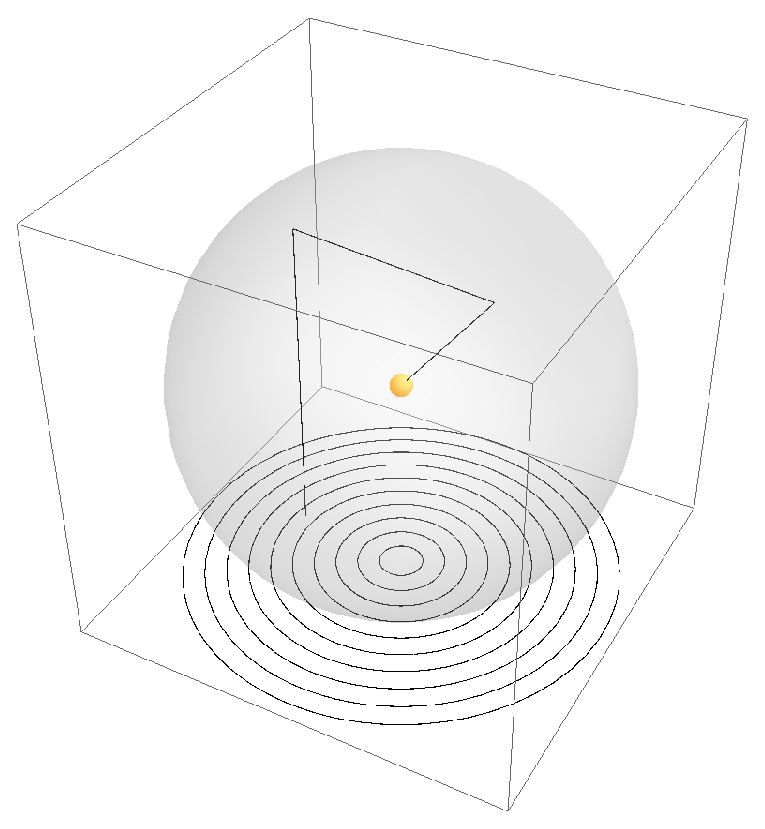
\includegraphics[height=0.3\textheight]{testproblem_illustration.eps}
			\caption{Illustration des Testproblems. Gezeigt ist ein Photonenpfad der zweimal gestreut wird und in einem ringf"ormigen Bin der orthographischen Kamera auftrifft}
			\label{fig:testproblem_sketch}
	\end{figure}

	
	\subsection{analytische L"osung}\label{subsec:homsphere_analytic_solution}
	\subsubsection{Green'sche Funktion f"ur den Photonentransport zwischen Kugelschalen}
	Um die korrekte radiale Intensit"atsverteilung zu berechnen, bestimmen wir zun"achst in Form der Green'schen Funktion $g$, wie sich die Photonen radial nach einem Streuvorgang ausgebreitet haben.
	Genauer gibt $g$ an, wie gro"s der Anteil der Photonen, die auf einer Kugelschale mit Radius $r_0$ starten, beim Radius $r_1$ w"ahrend des n"achsten Streuvorganges ist (siehe Abb. \ref{fig:radial_greens_function_pdfcdf}):
	\begin{align*}
		g(r_0,r_1) =& 2 \pi \int_0^\pi r_1^2 \sin(\theta) \frac{\exp\left(-\sqrt{r_0^2-2 r_0 r_1 \cos(\theta)+r_1^2}\right)}{4 \pi (r_0^2-2 r_0 r_1 \cos(\theta)+r_1^2)} \text{d}\theta \\
		=& \frac{1}{2}\frac{r_1}{r_0} \int_{|r_0-r_1|}^{r_0+r_1} \frac{e^{-t}}{t} dt \\
		=& \frac{1}{2}\frac{r_1}{r_0}\left[\text{Ei}(-(r_0+r_1)) - \text{Ei}(-|r_0-r_1|)\right]
	\end{align*}
	
	\begin{figure}
		\centering
		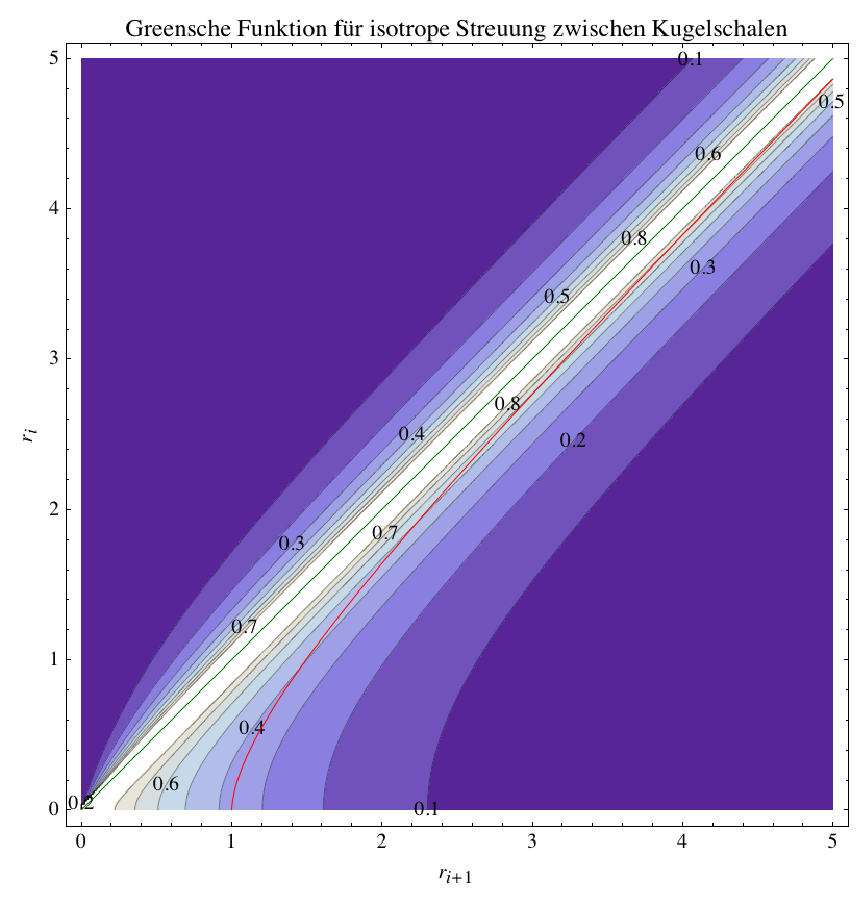
\includegraphics[width=0.48\textwidth]{radial_greens_function_pdf.eps}
		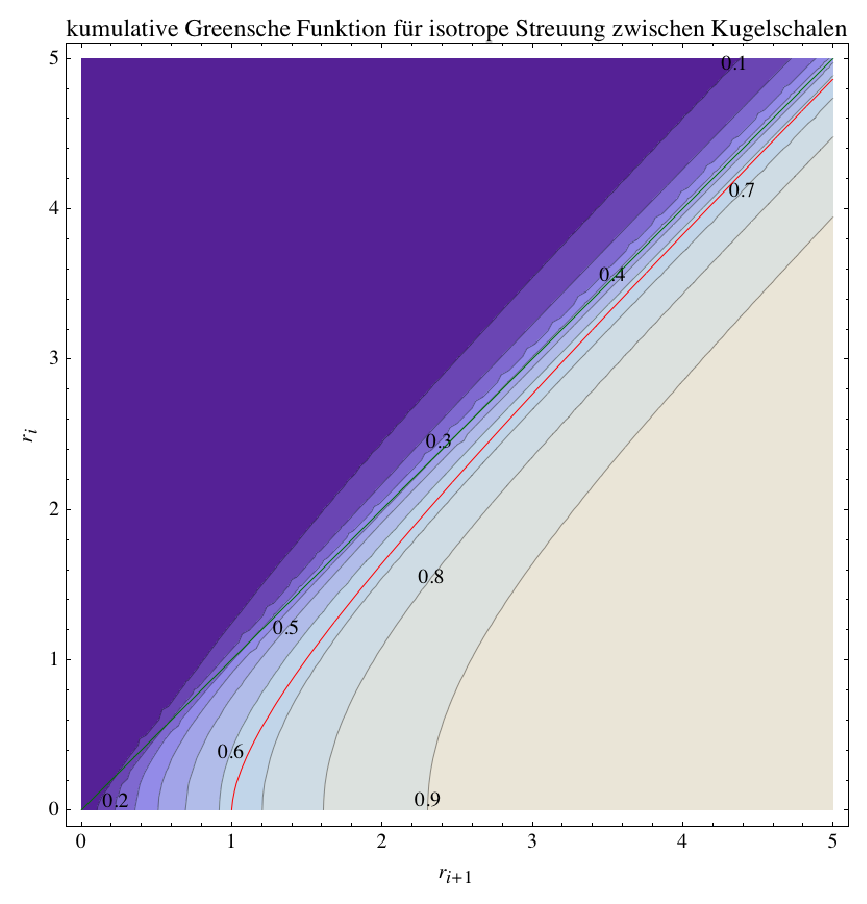
\includegraphics[width=0.48\textwidth]{radial_greens_function_cdf.eps}
		\caption{Green'sche Funktion der radialen Teilchenverteilung die von Radius $r_i$ kommen und beim Radius $r_{i+1}$ streuen als PDF und CDF. Der mittlere Radius ist in rot eingezeichnet.}
		\label{fig:radial_greens_function_pdfcdf}
	\end{figure}
	\begin{figure}
		\centering
		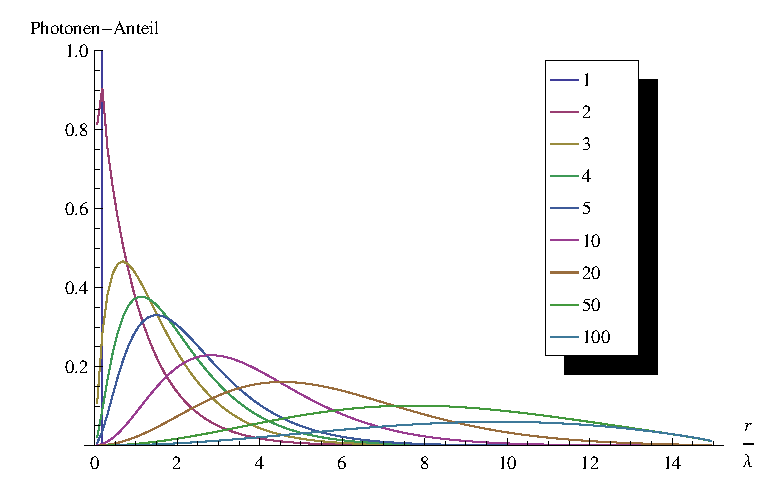
\includegraphics[width=0.9\textwidth]{gnlist_plot.eps}
		\caption{radiale Photonenverteilung nach n Streuvorg"angen. Die freie optische Wegl"ange ist dabei mit $\lambda=1/\sigma$ bezeichnet.}
		\label{fig:gnlist}
	\end{figure}
	Als n"achstes diskretisieren wir die Green'sche Funktion, indem wir ein gleichm"a"siges Gitter in $r_0$ und $r_1$ "uber $g$ legen, das sich bis zum Radius der Kugel $R$ erstreckt, und innerhalb jeder Gitterzelle $g$ in $r_0$--Richtung mitteln und in $r_1$--Richtung aufintegrieren und anschliessend die Ergebnisse in einer Matrix $\mathbf{g}$ speichern. Wenn wir nun einen Startvektor, der nur in der innersten Zelle von Null verschieden ist, $n$--mal mit $\mathbf{g}$ multiplizieren, bekommen wir die diskretisierte Photonenverteilung innerhalb der Kugelschalen beim $n$--ten Streuvorgang (siehe Abb. \ref{fig:gnlist}). Um die Emissivit"at $\varepsilon(r)$ jeder Kugelschale auszurechnen, summieren wir die Photonenverteilungen vom 1--ten bis zum $n$--ten Streuvorgang auf und teilen das Ergebnis in jeder Kugelschale durch ihr jeweiliges Volumen und den bestrahlten Raumwinkel $4\pi$. Die Intensit"aten k"onnen nun numerisch gem"a"s
	\begin{equation}
		I(r) = \int_{z=-h}^h \varepsilon\left(\sqrt{r^2+z^2}\right) e^{-(z+h)}\text{d}z\,,\quad h=\sqrt{R^2-r^2}
		\label{eq:testprob_intensity_calculation}
	\end{equation}
	berechnet werden.
	
	%\begin{figure}
	%	\centering
	%	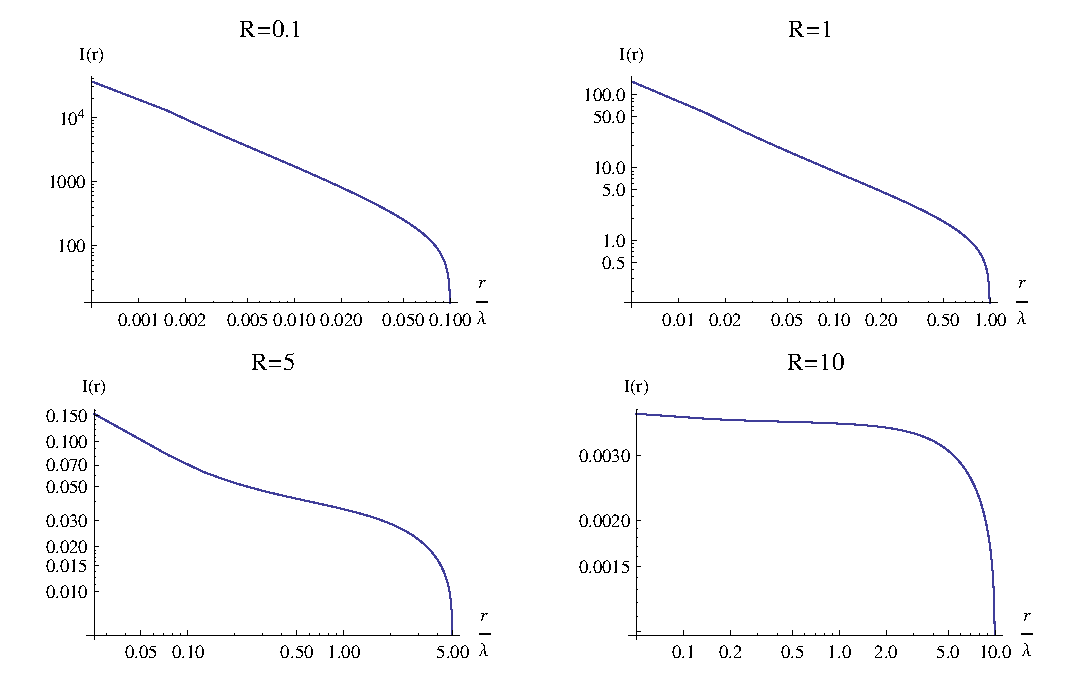
\includegraphics[width=1.0\textwidth]{analytical_tau_comparison.eps}
	%	\caption{radiales Intensit"atsprofil f"ur verschiedene Kugelradien und damit verschiedene optische Tiefen. $\lambda=1/\sigma$ bezeichnet die freie optische Wegl"ange.}
	%	\label{fig:analytical_tau_comparison}
	%\end{figure}
	
	%Das Ergebnis ist f"ur vier Kugelradien beispielhaft in Abb. \ref{fig:analytical_tau_comparison} dargestellt.
	
	\vfill
	\pagebreak
	\subsection{schnelle Monte--Carlo--L"osung}
	Eine andere Methode, schnell die radiale Intensit"atsverteilung zu bestimmen, ist durch folgendes Monte--Carlo--Schema gegeben:
	\begin{algorithmic}
		\STATE $M\leftarrow$ Anzahl Ringe
		\STATE $N\leftarrow$ Anzahl Photonen
		\STATE $R\leftarrow$ Kugelradius
		\FOR{$i=1$ to $N$}
			\STATE $\location{r}\leftarrow (0,0,0)^\text{T}$
			\REPEAT
				\STATE\COMMENT{w"ahle zuf"allige Richtung $\omega$}
				\STATE $z\leftarrow$ ziehe gleichf"ormig aus $[-1,1]$
				\STATE $\phi\leftarrow$ ziehe gleichf"ormig aus $[0,2\pi]$
				\STATE $s\leftarrow\sqrt{1-z^2}$
				\STATE $\omega\leftarrow (s\;\text{cos}(\phi),s\;\text{sin}(\phi),z)^\text{T}$
				\STATE\COMMENT{w"ahle exponentiell verteilte Entfernung $t$}
				\STATE $u\leftarrow$ ziehe gleichf"ormig aus $[0,1]$
				\STATE $t\leftarrow -\text{ln}(1-u)$
				\STATE $\location{r}_\text{old}\leftarrow\location{r}$
				\STATE $\location{r}\leftarrow\location{r}_\text{old}+\omega t$
			\UNTIL{$|\location{r}|\geq R$}
			\STATE\COMMENT{bestimme Sto"sparameter $b$}
			\STATE $\location{d}\leftarrow\location{r}-\location{r}_\text{old}$
			\STATE $b\leftarrow\sqrt{\langle\location{r},\location{r}\rangle-\frac{\langle\location{r},\location{d}\rangle}{\langle\location{d},\location{d}\rangle}}$
			\STATE $j\leftarrow\lfloor M\frac{b}{R}\rfloor$
			\STATE $C[j]=C[j]+1$
		\ENDFOR
		\FOR[normiere Bincounts mit Ringfl"achen]{$j=0$ to $M-1$}
			\STATE $C[j]=C[j]/(\pi R^2(2j+1)/M^2)$
		\ENDFOR
		\RETURN $C[\cdots]$
	\end{algorithmic}
	Dabei starten wir mit einem Photon im Ursprung und berechnen dann von der aktuellen Position solange die Position des n"achsten Streuereignisses, bis dieses ausserhalb der Kugel liegt. Damit kennen wir den letzten Streupunkt und die Richtung in die das Photon das Streuvolumen verl"asst. Da wir nur an der radialen Intensit"atsverteilung interessiert sind k"onnen wir die Symmetrie des Problems ausnutzen indem wir die Kamera immer so hindrehen, dass das entfliehende Photon senkrecht auf den (gedachten) Sensor auftrifft. Das bedeutet, dass nicht die genaue Entweichrichtung sondern nur der Sto"sparameter entscheidend ist. Mit diesem Trick k"onnen wir jedes entweichende Photon z"ahlen, sodass dieses Verfahren sehr schnell konvergiert.
	
	
	\subsection{Resultate}
	Um die korrekte Berechnung des Strahlungstransports "uberpr"ufen zu k"onnen, simulieren wir das vorgestellte Problem der homogen streuenden Kugel f"ur drei verschiedene Radien (und damit optische Tiefen) jeweils mit der in Abschnitt~\ref{subsec:homsphere_analytic_solution} vorgestellten Methode, die wir als Referenzl"osung benutzen. Dieselben Konfigurationen berechnen wir au"serdem mit \texttt{MC3D} und \texttt{PIRaTE}. Von \texttt{MC3D} lassen wir hierf"ur $3.6\cdot10^8$ Photonen generieren und von 72 virtuellen Kameras, die auf einem Kreis auf das Zentrum blickend im Abstand von 5 Grad verteilt sind, beobachten. Jede Kamera ist dabei in einem Kegel mit "Offnungswinkel von $\alpha=5^\circ$ f"ur eintreffende Photonen empfindlich\footnote{In Abb.~\ref{fig:alphacomparison} ist der Effekt unterschiedlicher Kamera"offnungswinkel $\alpha$ bei gleicher Photonenanzahl gezeigt.}. \texttt{PIRaTE} benutzt eine einzige Kamera deren Empfindlichkeitskegel einen "Offnungswinkel von $30'$ besitzt. Hier generieren wir die Bilder in mehreren unabh"angigen L"aufen mit Pfadanzahlen zwischen $10^5$ und $10^7$.
	
		\begin{figure}
			\centering
			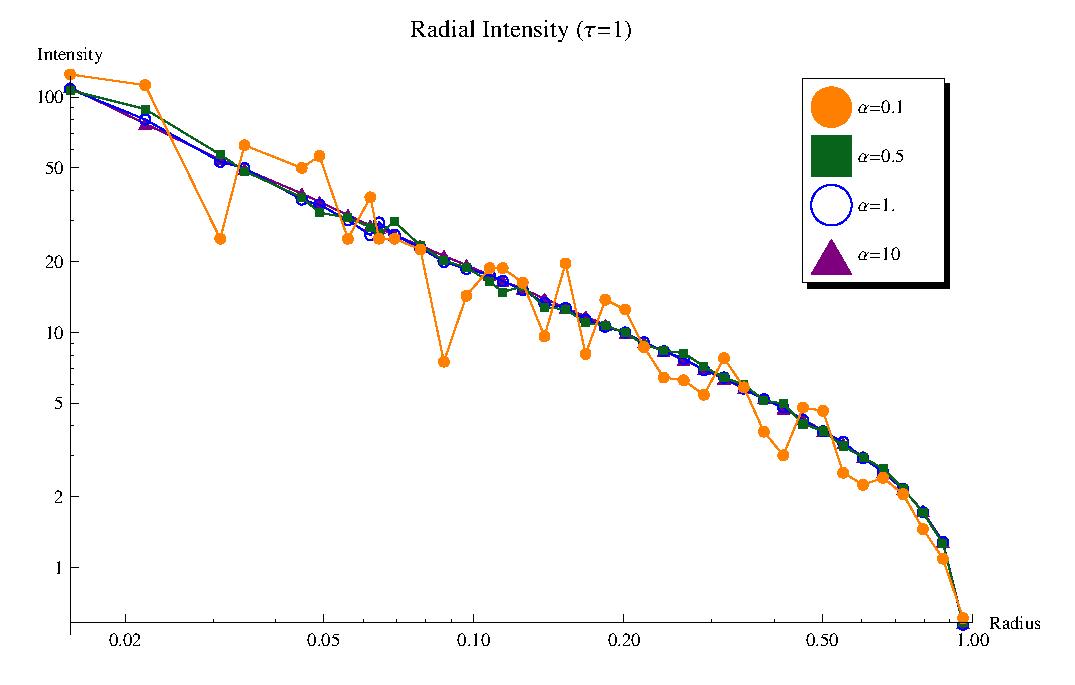
\includegraphics[width=0.8\textwidth]{mc3dalphasplot.eps}
			\caption{Radiale Intensit"atsprofile auf der Grundlage von \texttt{MC3D}--Simulationen --- Bei gleicher Photonenzahl aber sinkendem Kamera--"Offnungswinkel $\alpha$ steigt der statistische Fehler aufgrund der geringeren Zahl beachteter Photonen.}
			\label{fig:alphacomparison}
		\end{figure}
		
	Die drei zur Simulation gew"ahlten optischen Tiefen $\tau\in\{0.01,1,10\}$ decken den optisch d"unnen, mittleren und dicken Fall ab.	In Abb.~\ref{fig:methodcomparisongraphics} sind mit der analytischen Methode, \texttt{MC3D} und \texttt{PIRaTE} gewonnene radiale Intensit"atsprofile abgebildet.
	Im dargestellten Bereich stimmen die Ergebnisse beider Programme im Rahmen des statistischen Fehlers gut mit der analytischen L"osung "uberein. Dabei ist zu bedenken, dass bei kleineren Radien "uber weniger Pixel der zugrundeliegenden Bilder gemittelt wird und somit der statistische Fehler dort naturgem"a"s gr"o"ser ausf"allt.
		\begin{figure}
			\centering
			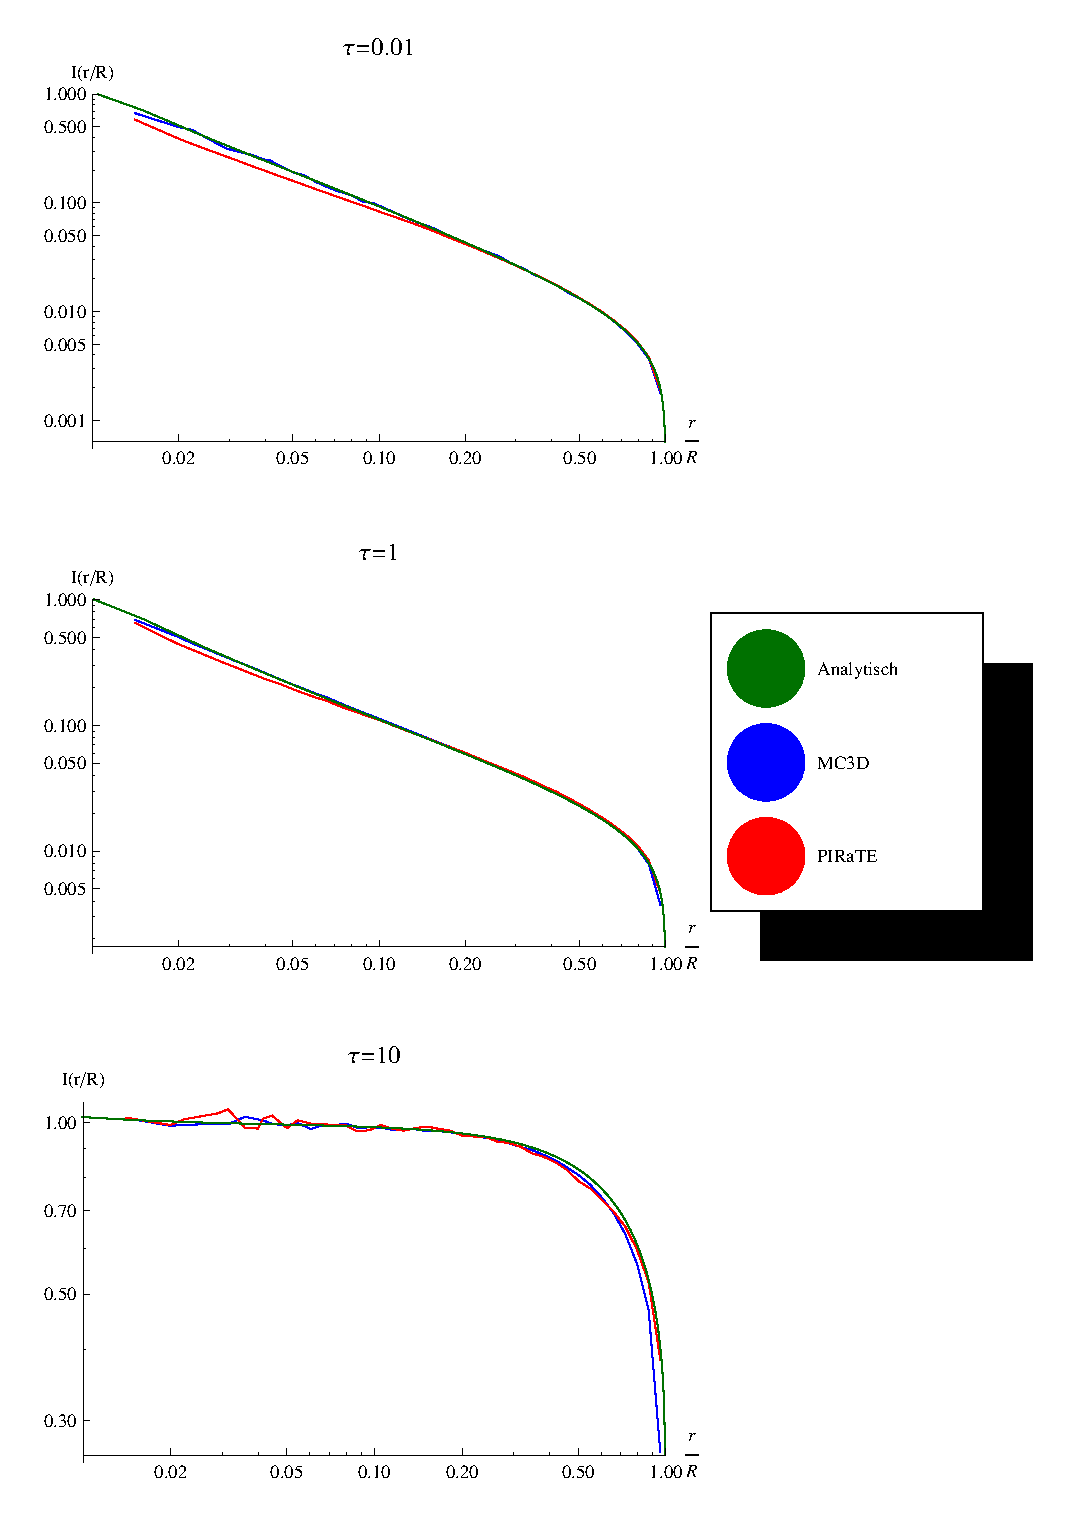
\includegraphics[height=1.0\textheight]{methodcomparisongraphics.eps}
			\caption{Vergleich zwischen der analytischen L"osung, \texttt{MC3D} und \texttt{PIRaTE} bei verschiedenen optischen Tiefen. \texttt{MC3D} hat f"ur alle drei F"alle $3.6\cdot10^8$ Photonen, \texttt{PIRaTE} jeweils $4.88\cdot10^7,4.88\cdot10^7,2.088\cdot10^8$ Photonenpfade generiert.}
			\label{fig:methodcomparisongraphics}
		\end{figure}
	
	Bei Betrachtung von horizontalen Schnitten durch die Streubilder (siehe Abb.~\ref{fig:sphere_image_cuts}) f"allt auf, das \texttt{PIRaTE} den Anteil des direkt von der Punktlichtquelle kommenden Lichtes falsch sch"atzt. Dies liegt vermutlich an den Sensorparametern (insbesondere dem "Offnungswinkel), da im Unterschied zu \texttt{MC3D} in \texttt{PIRaTE} keine punktf"ormigen sondern nur ausgedehnte Lichtquellen existieren, die bei kleinen Ausma"sen mit der jetzigen Pfadgenerierungsmethode schwer zu samplen sein k"onnen. Zur end"ultigen Kl"arung bedarf es aber einer genaueren Fehleranalyse.
	
		\begin{figure}
			\centering
			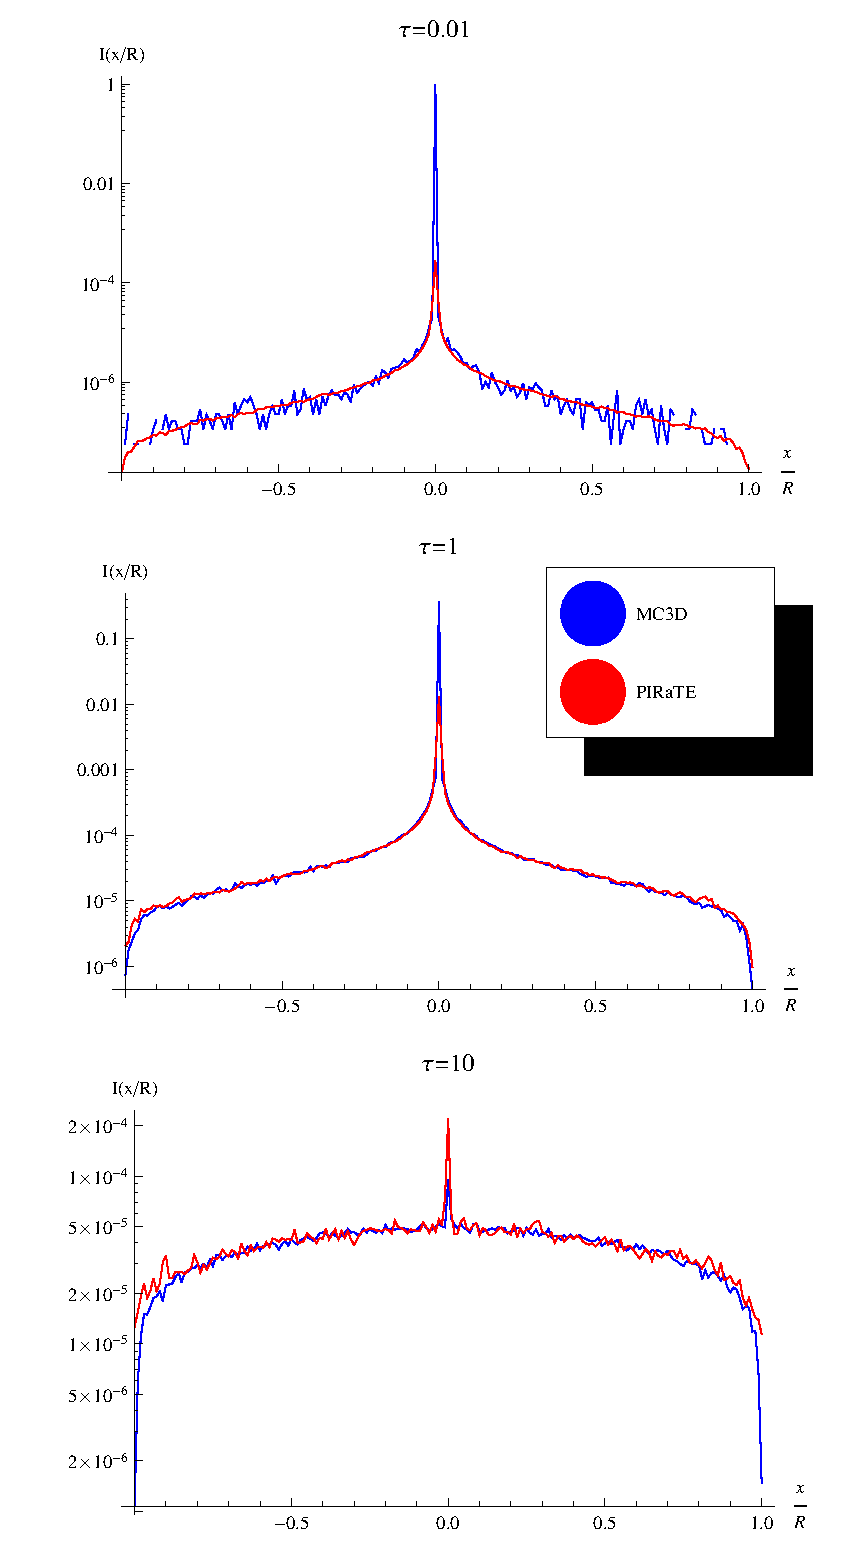
\includegraphics[height=1.0\textheight]{sphere_image_cuts.eps}
			\caption{Horizontale Schnitte durch die Streubilder f"ur die drei optischen Tiefen bei hoher Anzahl an Photonen bzw. Pfade.}
			\label{fig:sphere_image_cuts}
		\end{figure}
	
	Um nicht komplett auf einen Vergleich der Konvergenzraten beider Programme verzichten zu m"ussen, verwenden wir zur Berechnung der Abweichung vom Referenzbild maskierte Bilder, bei denen die Lichtquelle in der Mitte des Bildes ausgeblendet ist.	 Die Referenzbilder %(siehe Abb.~\ref{fig:sphere_reference_images}) 
	werden dabei aus den, aus allen 72 Kameraebenen akkumulierten, von \texttt{MC3D} erzeugten Streubildern generiert. Zus"atzlich mitteln wir innerhalb des Bildes "uber alle Pixelgruppen mit exakt gleichem Abstand vom Zentrum% (siehe Abb.~\ref{fig:polaraveragingsymmetry})
	. Dies f"uhrt im Durchschnitt zu einer Mittelung "uber 11 Pixel wodurch das Rauschen ungef"ahr gedrittelt wird, was insbesondere bei dem Bild der optisch d"unnen Kugel, welches das st"arkste Rauschen besitzt, hilfreich ist.
	
		%\begin{figure}
		%	\centering
		%	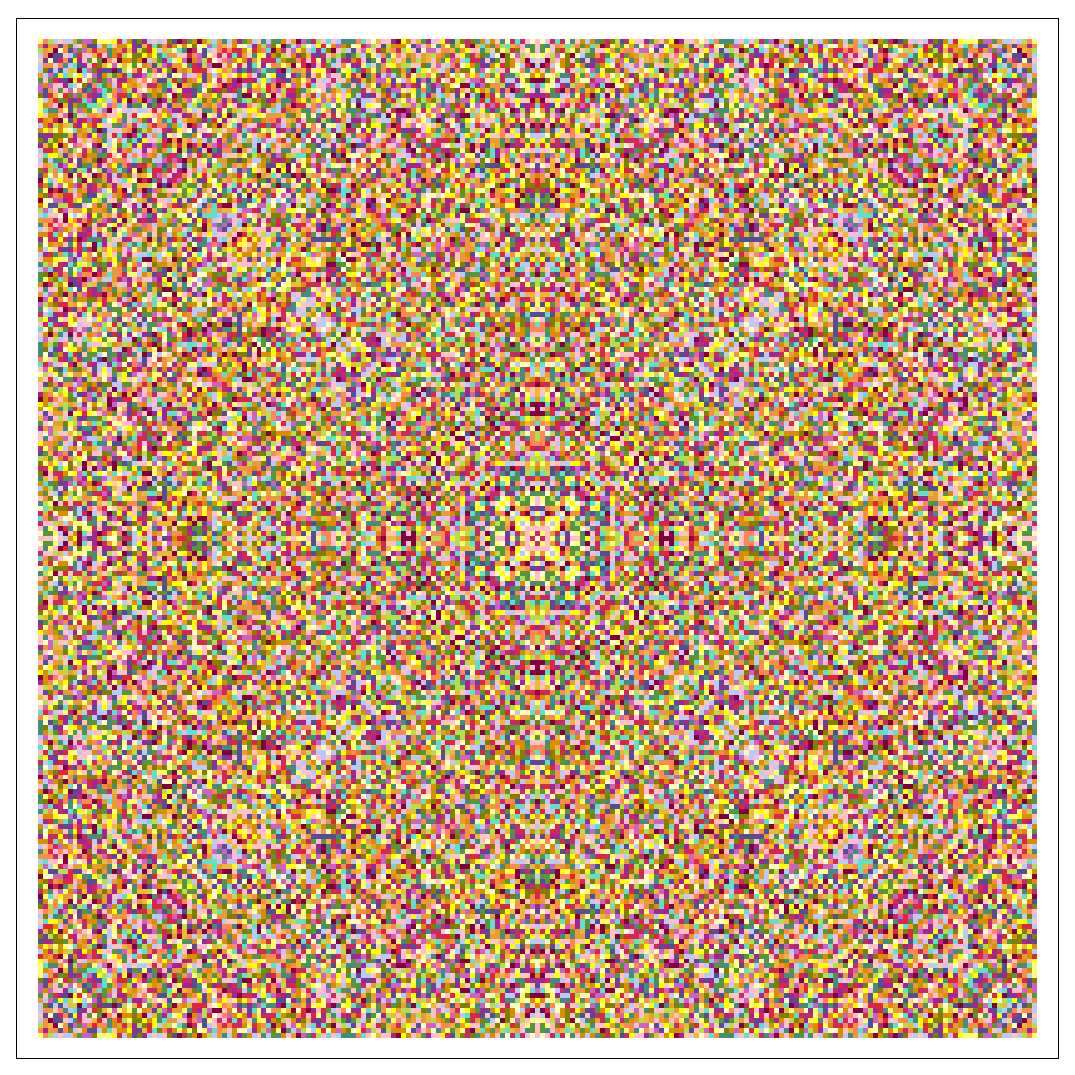
\includegraphics[width=0.5\textwidth]{polaraveragingsymmetry.eps}
		%	\caption{Darstellung der Symmetrien, die bei der polaren Mittelung genutzt werden. Pixel mit exakt gleichem Abstand zum Zentrum sind gleich gef"arbt. Im Schnitt wird "uber 11 Pixel gemittelt.}
		%	\label{fig:polaraveragingsymmetry}
		%\end{figure}
		
		%\begin{figure}
		%	\centering
		%	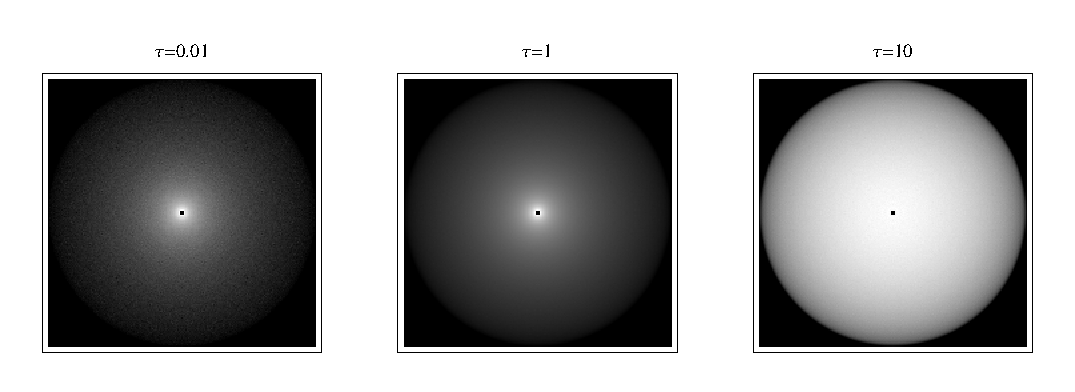
\includegraphics[width=1.0\textwidth]{spherereferenceimages.eps}
		%	\caption{Referenzbilder zur Bestimmung der Abweichungen}
		%	\label{fig:sphere_reference_images}
		%\end{figure}
	
	Eine Auswahl der generierten Streubilder ist in den Abbildungen \ref{fig:mc3d_sphere_imageoverview} und \ref{fig:pirate_sphere_imageoverview} dargestellt und jeweils mit der Anzahl an generierten Photonen bzw. Pfaden sowie der zum generieren ben"otigten Rechenzeit versehen. Die \texttt{MC3D}--Rechenzeiten sind trotz unterschiedlicher Photonenzahlen konstant. Dies liegt daran, dass die Bilder nur unterschiedlich viele aufsummierte Kameraebenen desselben Simulationslaufes darstellen und nicht die Summe der Ergebnisse verschiedener Simulationen.
	
	Aufgrund der unterschiedlichen zugrundeliegenden Algorithmen, Programmiersprachen, Compiler und Computer mit denen die Ergebnisse erzeugt wurden, ist es schwierig die beiden Programme objektiv zu vergleichen. W"ahrend \texttt{MC3D} eine feste Zahl von Photonen simuliert, die entweder in einer Kameraebene aufgefangen und gez"ahlt werden oder nicht, generiert \texttt{PIRaTE} eine feste Zahl Pfade, die den Sensor erreicht haben aber unterschiedlich stark gewichtet in das Ergebnis eingehen. W"ahrend \texttt{MC3D} immer von einer inhomogenen Dichteverteilung ausgeht und aufintegriert, um optische Tiefen zu bestimmen, kann \texttt{PIRaTE} die optischen Tiefen im homogenen Fall direkt berechnen. \texttt{MC3D} generierte die Ergebnisse auf einem Intel Xeon E5405 (2000 MHz) Prozessor--Kern, \texttt{PIRaTE} auf einem AMD Opteron 8354 (2200 MHz) Prozessor--Kern. Daher sollten die Ergebnisse als Gr"ossenordnungsabsch"atzungen und nicht als absolut unumst"o"sliche Messergebnisse interpretiert werden.
	
		\begin{figure}
			\centering
			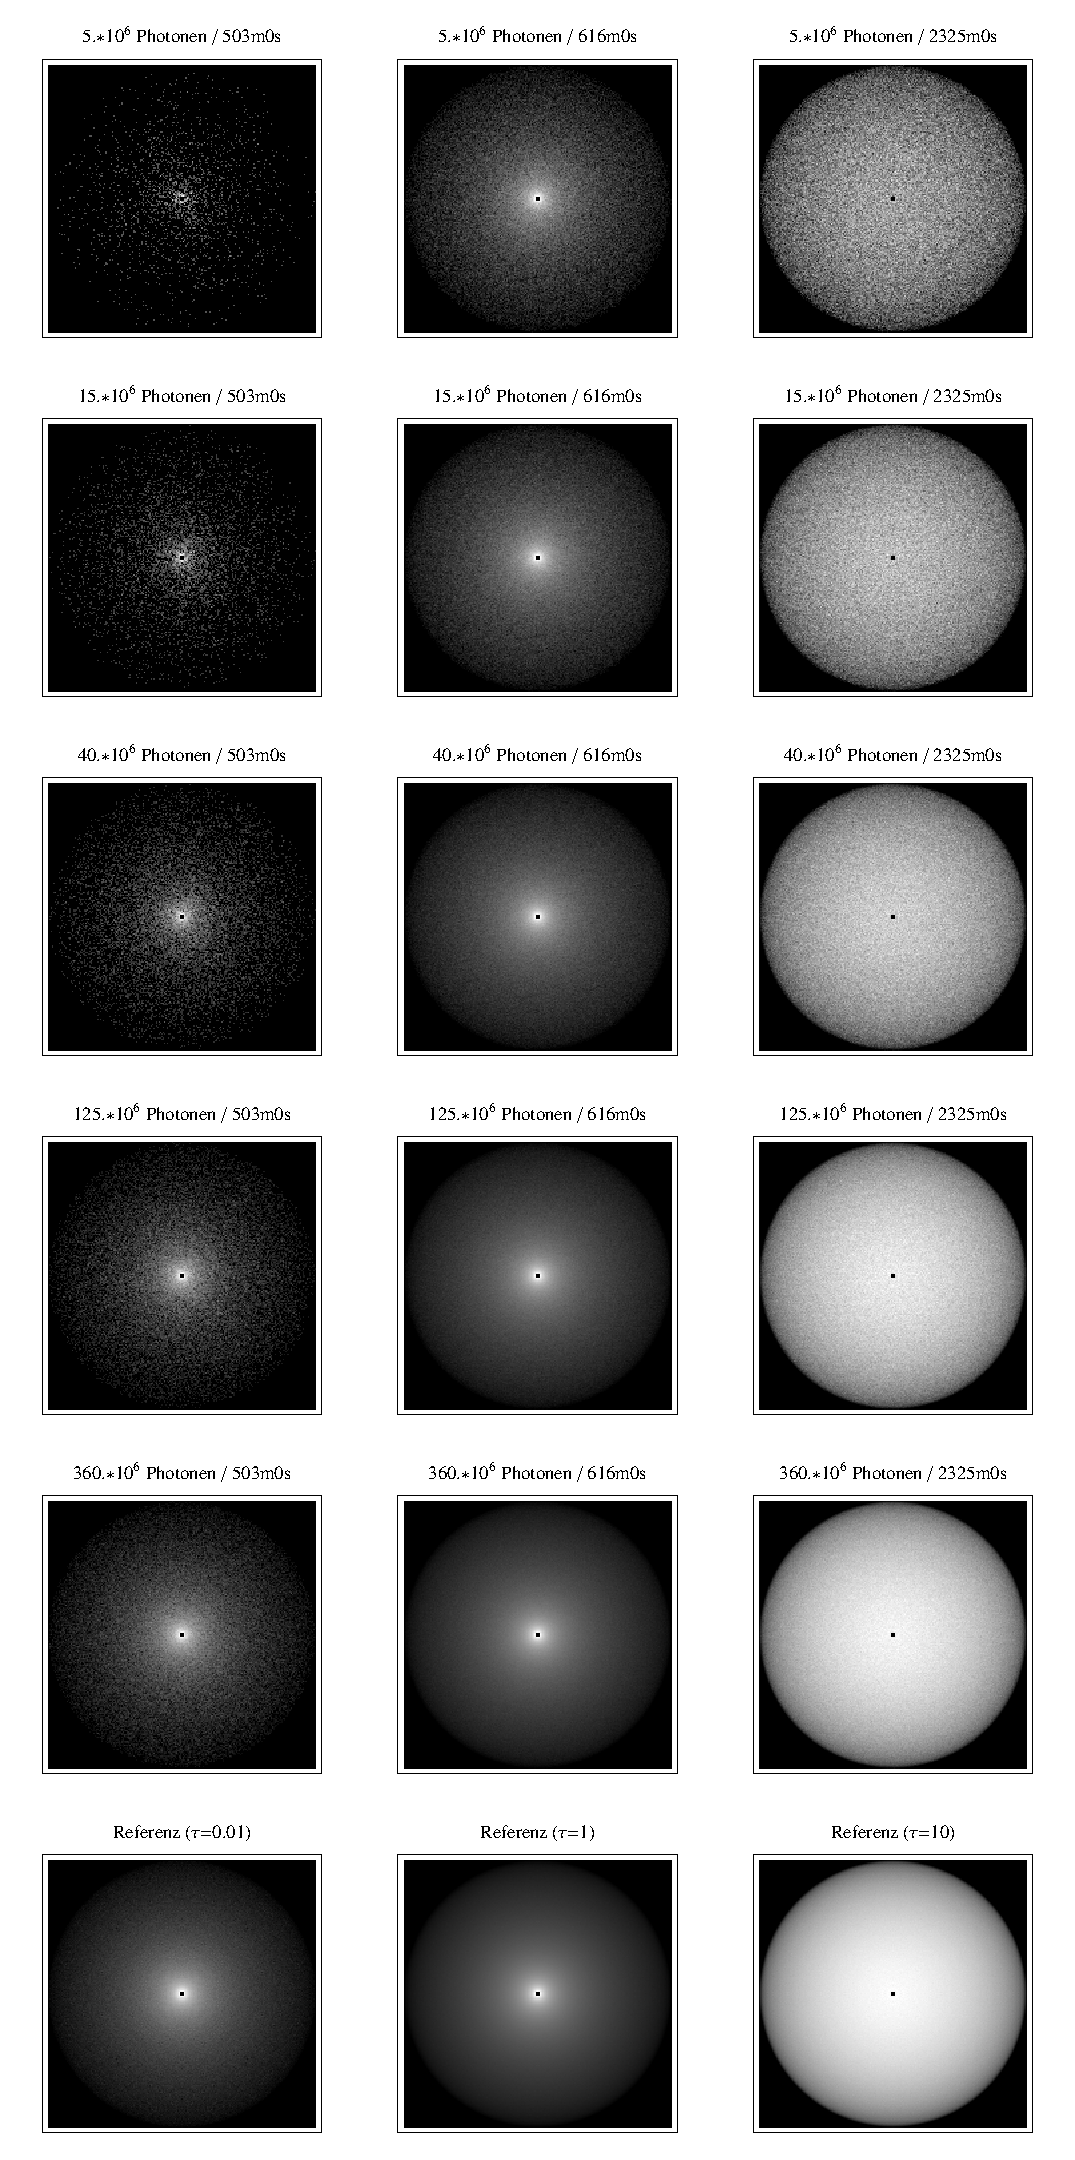
\includegraphics[height=1.0\textheight]{mc3dsphereimageoverview.eps}
			\caption{"Ubersicht "uber die Qualit"at der Bilder bei Akkumulation unterschiedlich vieler Kameraebenen der \texttt{MC3D}--Simulationen und der Simulationszeiten.}
			\label{fig:mc3d_sphere_imageoverview}
		\end{figure}
		\begin{figure}
			\centering
			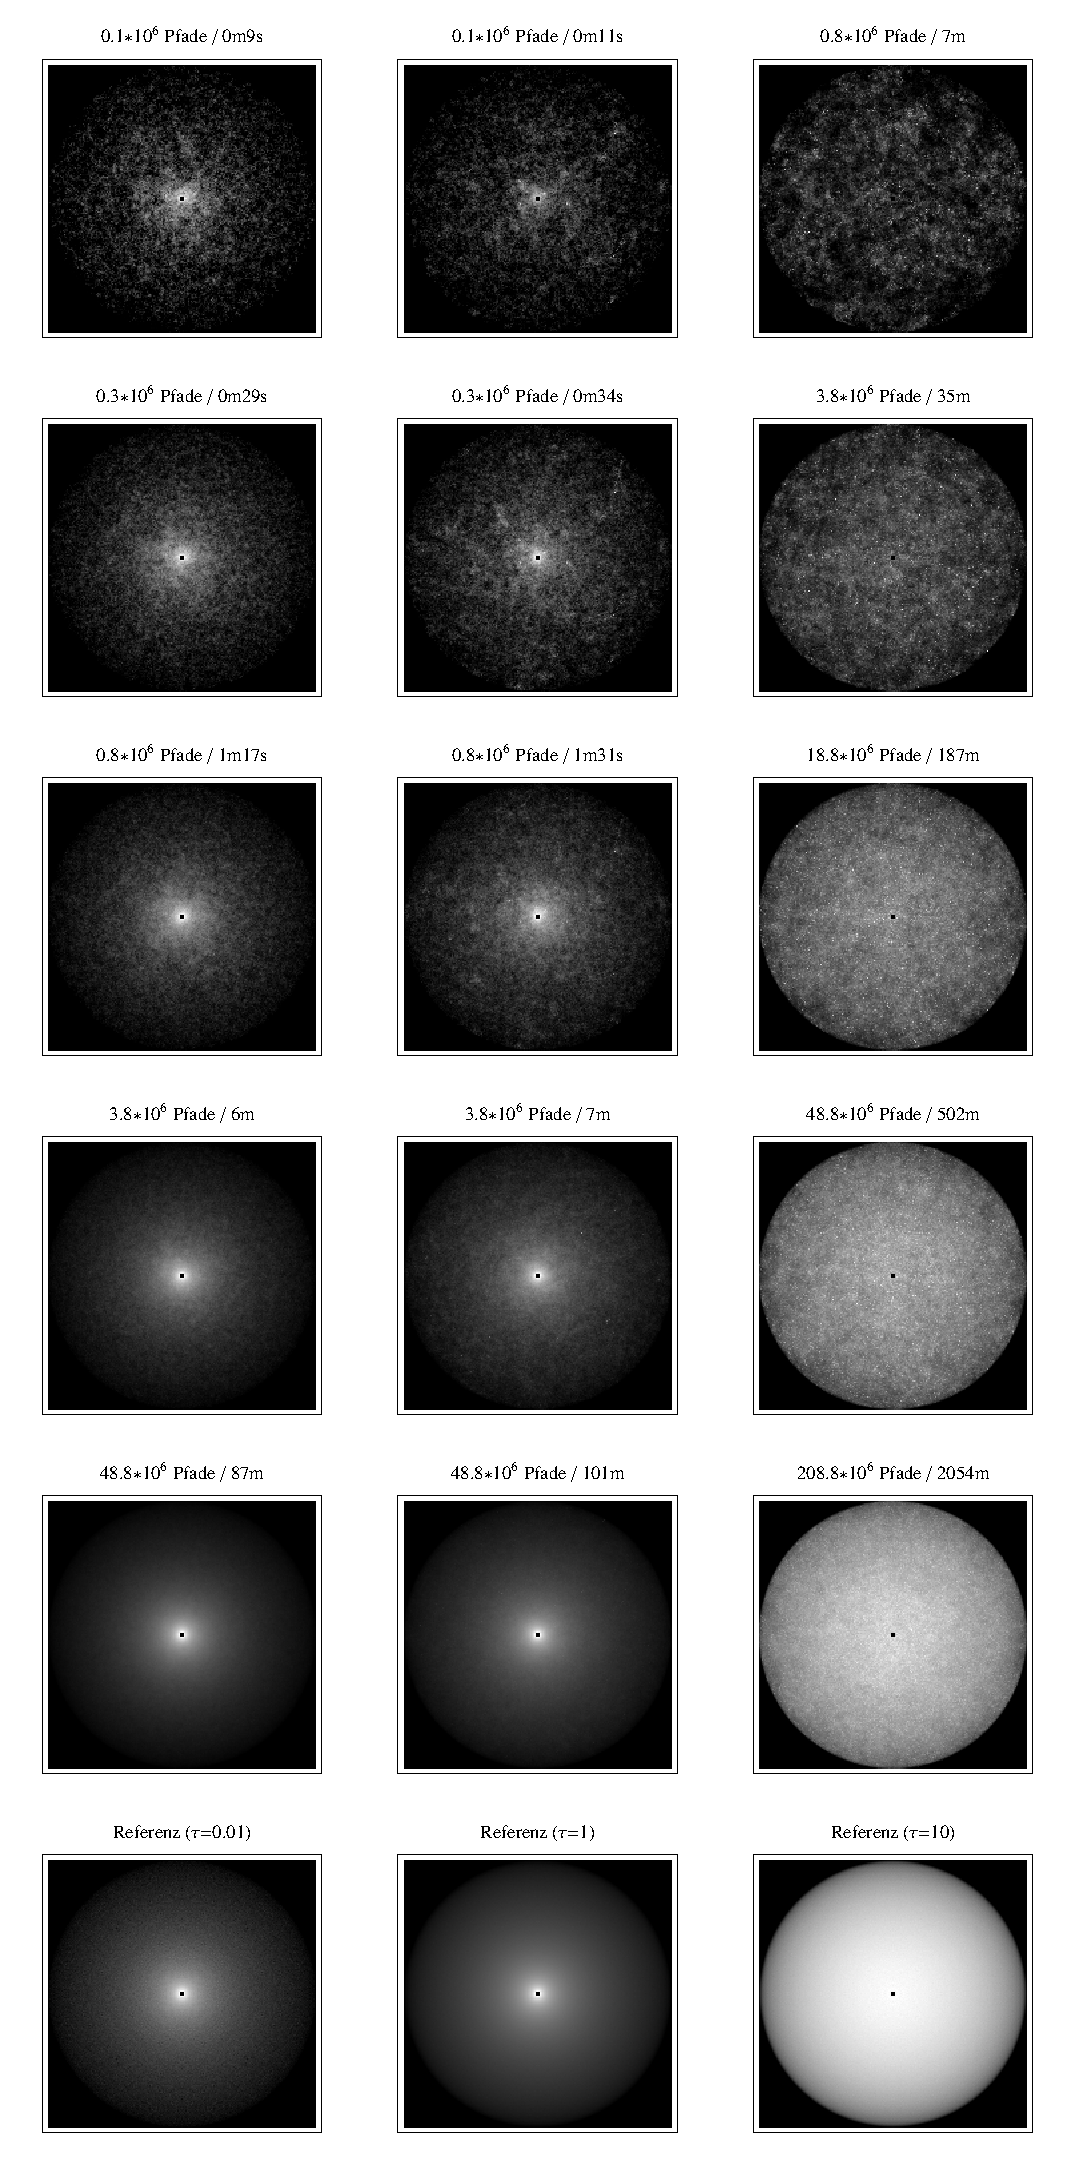
\includegraphics[height=1.0\textheight]{piratesphereimageoverview.eps}
			\caption{"Ubersicht "uber die Qualit"at der Bilder bei unterschiedlich langen \texttt{PIRaTE}--Simulationsl"aufen.}
			\label{fig:pirate_sphere_imageoverview}
		\end{figure}
	
	
	In Abb.~\ref{fig:sphere1_error}-\ref{fig:sphere3_error} sind f"ur die verschiedenen optischen Tiefen jeweils der absolute sowie der relative Fehler zum Referenzbild gegen die Anzahl berechneter Photonen/Pfade bzw. die Rechenzeit aufgetragen. Der absolute Fehler wird als mittlerer quadratischer Fehler aller Pixel berechnet. Zur Berechnung des relativen Fehlers wurde dabei die Methode von \citet{Pryce:1984p13059} verwendet. Da bei \texttt{MC3D} die verschiedenen Streubilder nicht durch mehrere Simulationsl"aufe sondern mehrere Kameraebenen erzeugt wurden, sind f"ur \texttt{MC3D} zwei Kurven eingezeichnet. Beide Kurven fassen die Summation unterschiedlich vieler Kameraebenen der durchgef"uhrten Simulation als die Ergebnisse verschiedener Simulationen mit unterschiedlicher Anzahl generierter Photonen aber konstanter Kameraebenenanzahl auf. Die linke Kurve interpretiert sie als die Ergebnisse einer Simulation mit 72, die rechte als Ergebnis einer Simulation mit nur einer Kameraebenen auf.
	
	Im optisch d"unnen Fall ($\tau=0.01$, Abb.~\ref{fig:sphere1_error}) erzeugt \pirate mit einer Gr"o"senordnung weniger Pfaden Bilder gleichen Fehlers. Bei nur einer Kameraebene sind es sogar drei Gr"o"senordnungen. Die Abflachung der Konvergenzrate von \pirate liegt daran, dass dort der Fehler der Simulationen unter den Rauschpegel der Referenzbilder f"allt. Zur h"oheren Effizienz tr"agt vermutlich zum Gro"steil der verwendeten Distanzsampler (siehe Gleichung \ref{eq:enforced_scattering_distancesampler}) bei, der eine (in diesem Fall seltene) Streuung erzwingt.

		\begin{figure}
			\centering
			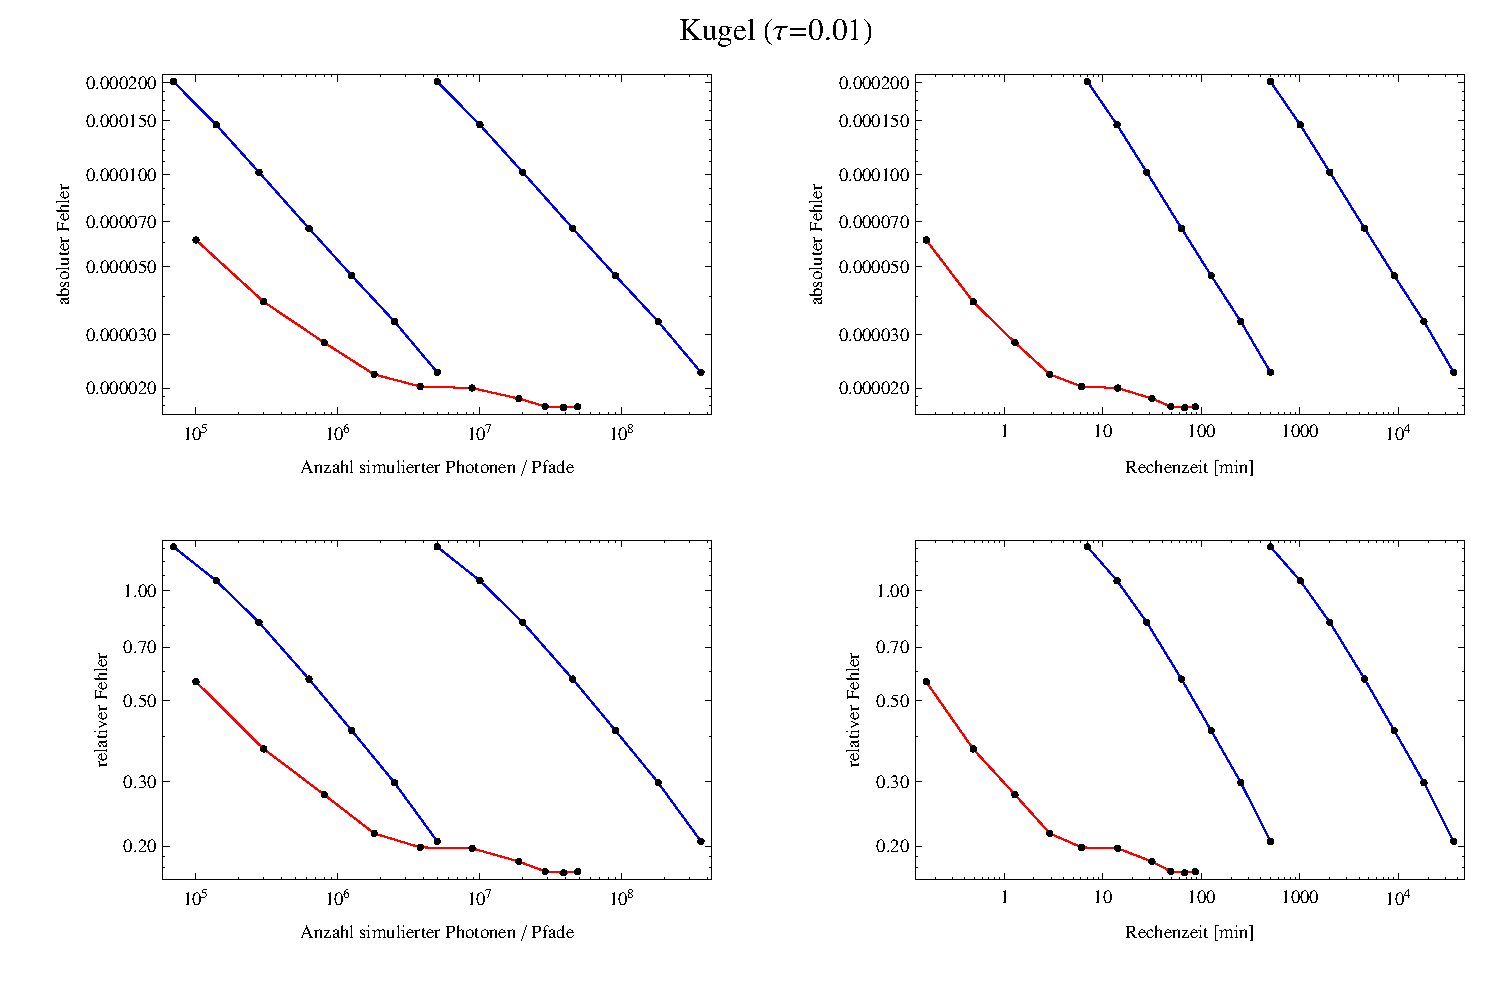
\includegraphics[angle=90,height=1.0\textheight]{sphere1errorplot.eps}
			\caption{Die blauen Linien repr"asentieren \texttt{MC3D}, wobei daf"ur die Bilder aus (1,2,4,9,18,36,72) Kameraebenen aufsummiert wurden. Die Schr"age Linie extrapoliert, wie aufw"andig die Simulation mit nur einer Kameraebene gewesen w"are.}
			\label{fig:sphere1_error}
		\end{figure}
		\begin{figure}
			\centering
			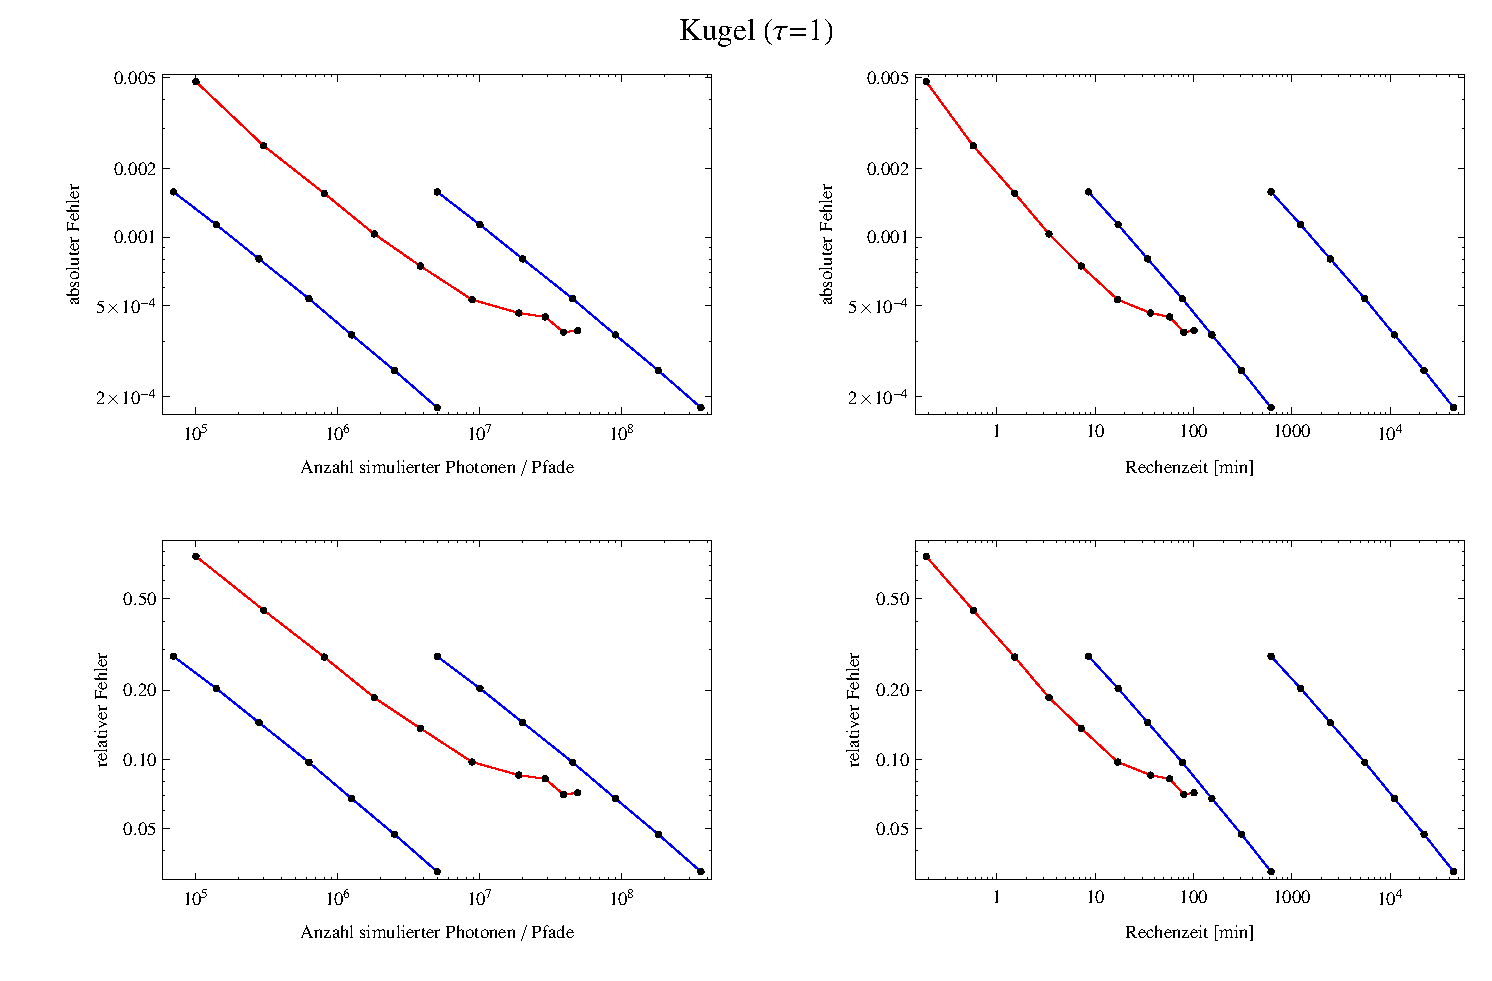
\includegraphics[angle=90,height=1.0\textheight]{sphere2errorplot.eps}
			\caption{Die blauen Linien repr"asentieren \texttt{MC3D}, wobei daf"ur die Bilder aus (1,2,4,9,18,36,72) Kameraebenen aufsummiert wurden. Die Schr"age Linie extrapoliert dabei, wie aufw"andig die Simulation mit nur einer Kameraebene gewesen w"are.}
			\label{fig:sphere2_error}
		\end{figure}
		\begin{figure}
			\centering
			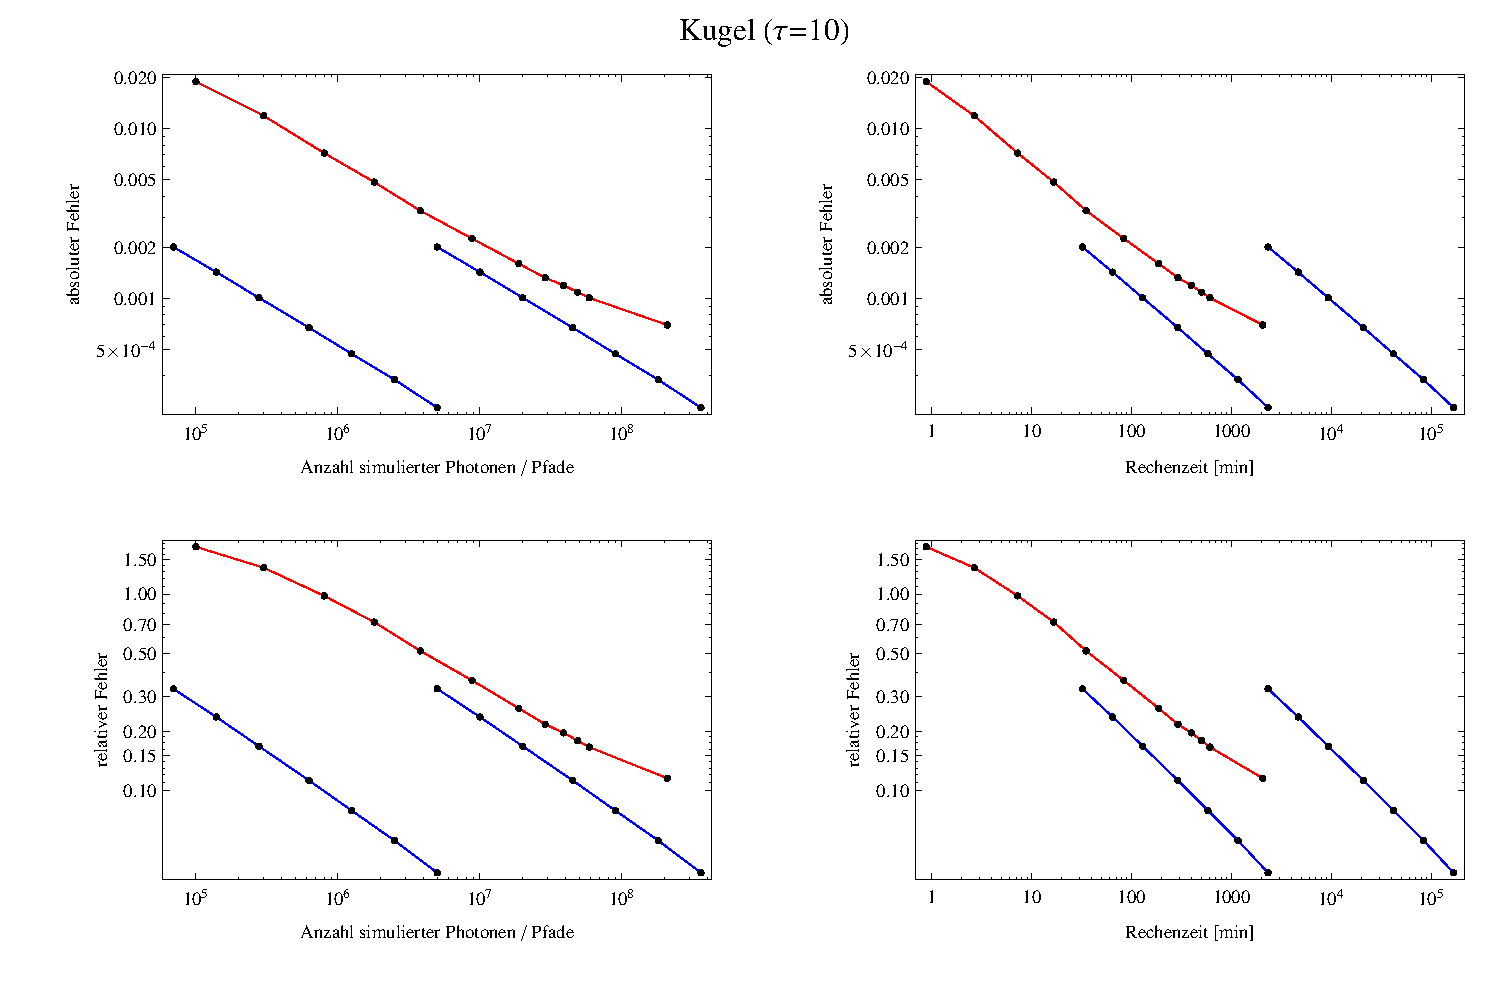
\includegraphics[angle=90,height=1.0\textheight]{sphere3errorplot.eps}
			\caption{Die blauen Linien repr"asentieren \texttt{MC3D}, wobei daf"ur die Bilder aus (1,2,4,9,18,36,72) Kameraebenen aufsummiert wurden. Die Schr"age Linie extrapoliert dabei, wie aufw"andig die Simulation mit nur einer Kameraebene gewesen w"are.}
			\label{fig:sphere3_error}
		\end{figure}
	
	\section{Einfaches Scheibenmodell}
	TODO: Formel und KonturPlot f"ur Dichteverteilung.
	\subsection{Resultate}
	TODO: Konvergenz--Geschwindigkeits--Vergleich mit MC3D.
	Stichpunkte:tau=97.6958 in der Mittelebene. 1m55s f"ur $10^6$ Photonen mit MC3D. 720M Photonen in 72Ebenen $\rightarrow$ Jede Ebene entspricht 10M Photonen
	\section{Einordnung der Resultate}
	TODO: Gesamtvergleich zwischen MC3D und PIRaTE: PIRaTE schneller, MC3D nat"urlicheres Rauschen, PIRaTE bedarf weiterer Kalibration f"ur ZentralSternIntensit"at